\documentclass[12pt]{article}

%Paquetes
\usepackage[left=2cm,right=2cm,top=3cm,bottom=3cm,letterpaper]{geometry}
\usepackage{lmodern}
\usepackage[T1]{fontenc}
\usepackage[utf8]{inputenc}
\usepackage[spanish,activeacute]{babel}
\usepackage{mathtools}
\usepackage{amssymb}
\usepackage{enumerate}
\usepackage{tabularx}
\usepackage{wasysym}
\usepackage{listings}
\usepackage{graphicx}

%\usepackage{graphicx}
%\graphicspath { {tarea01/media/} }
%\usepackage{pifont}

%Preambulo
\title{Tecnologías para desarrollos en internet \\ Manual CRUD: Beego}
\author{Kihui-DEV}
\date{Fecha: 18/09/16 \\ Facultad de Ciencias UNAM}

\begin{document}
\maketitle
Agregar índice.
\section*{Introducción}
\section*{Instalación de GO}
\subsection*{Descarga y configuración}
Para obtener el paquete de Golang y descomprimirlo \\
Ejecutar:
\begin{verbatim}
  $ wget https://golang.org/doc/install?download=go1.7.1.linux-amd64.tar.gz

  # tar -C /usr/local -xzf go1.7.1.linux-amd64.tar.gz
\end{verbatim}


Agregar esta línea en el script de inicio (típicamente en \textit{/user/local/profile}
si se desea hacer una instalación general en el sistema operativo o
en en particular para el usuario en curso \textit{\~/.profile}):
\begin{verbatim}
  export PATH=$PATH:/usr/local/go/bin
\end{verbatim}

\subsection*{Prueba}
Crear un directorio que haga de workspace para la prueba.\\
Por ejemplo:
\begin{verbatim}
  $ mkdir ~/go
\end{verbatim}
Asignar la variable \textbf{GOPATH} para que apunte a tal dirección:
\begin{verbatim}
  $ export GOPATH=$HOME/go
\end{verbatim}
Bien podemos hacer persistente este cambio agregando la misma línea al script
de inicio que editamos en la sección anterior (ir a Descarga y configuración). \par

A continuación, creamos dentro de ese directorio  \textit{src/hola}.
Y dentro de \textit{hola\/} un fichero nuevo de nombre \textit{hola.go}:
\begin{verbatim}
     package main

     import "fmt"

     func main() {
         fmt.Printf("hola, mundo\n")
     }
\end{verbatim}

Luego, desde cualquier ubicación podemos ejecutar\\
esto:
\begin{verbatim}
  $ go install hola
\end{verbatim}

Esto producirá un ejecutable \textit{hola} dentro de el directorio \textit{go/bin/},
que podemos ejecutar utilizando lo siguiente:
\begin{verbatim}
  $ $GOPATH/bin/hola
\end{verbatim}

Si produce la salida ``hola, mundo'', quiere decir que nuestra instalación fue exitosa.

\section*{Instalación de Beego}

\noindent Para instalar Beego utilizamos el siguiente comando:
\begin{verbatim}
$ go get github.com/astaxie/beego
\end{verbatim}

\noindent Para compilar y correr nuestros proyectos necesitaremos instalar Bee también:
\begin{verbatim}
$ go get github.com/beego/bee
\end{verbatim}

\noindent Para crear un proyecto en Beego, necesitamos ir al directorio de nuestro $\$$GOPATH, donde escribimos el siguiente comando:
\begin{verbatim}
$ bee new quickstart
\end{verbatim}
\noindent Podremos ver que se han creado las sigueintes carpetas y archivos necesarios para nuestra aplicación:

\begin{verbatim}
quickstart
|-- conf
|   |__ app.conf
|-- controllers
|   |__ default.go
|-- main.go
|-- models
|-- routers
|   |__ router.go
|-- static
|   |--- css
|   |--- img
|   |__ js
|-- tests
|   |__ default_test.go
|-- views
    |__ index.tpl
\end{verbatim}

\noindent Finalmente para correr el nuevo proyecto que hemos creado,  hacemos lo siguiente:
\begin{verbatim}
$ cd quickstart
$ bee run
\end{verbatim}
\noindent Y si entramos a localhost:8080 desde nuestro navegador podemos ver la siguiente página de inicio: \\

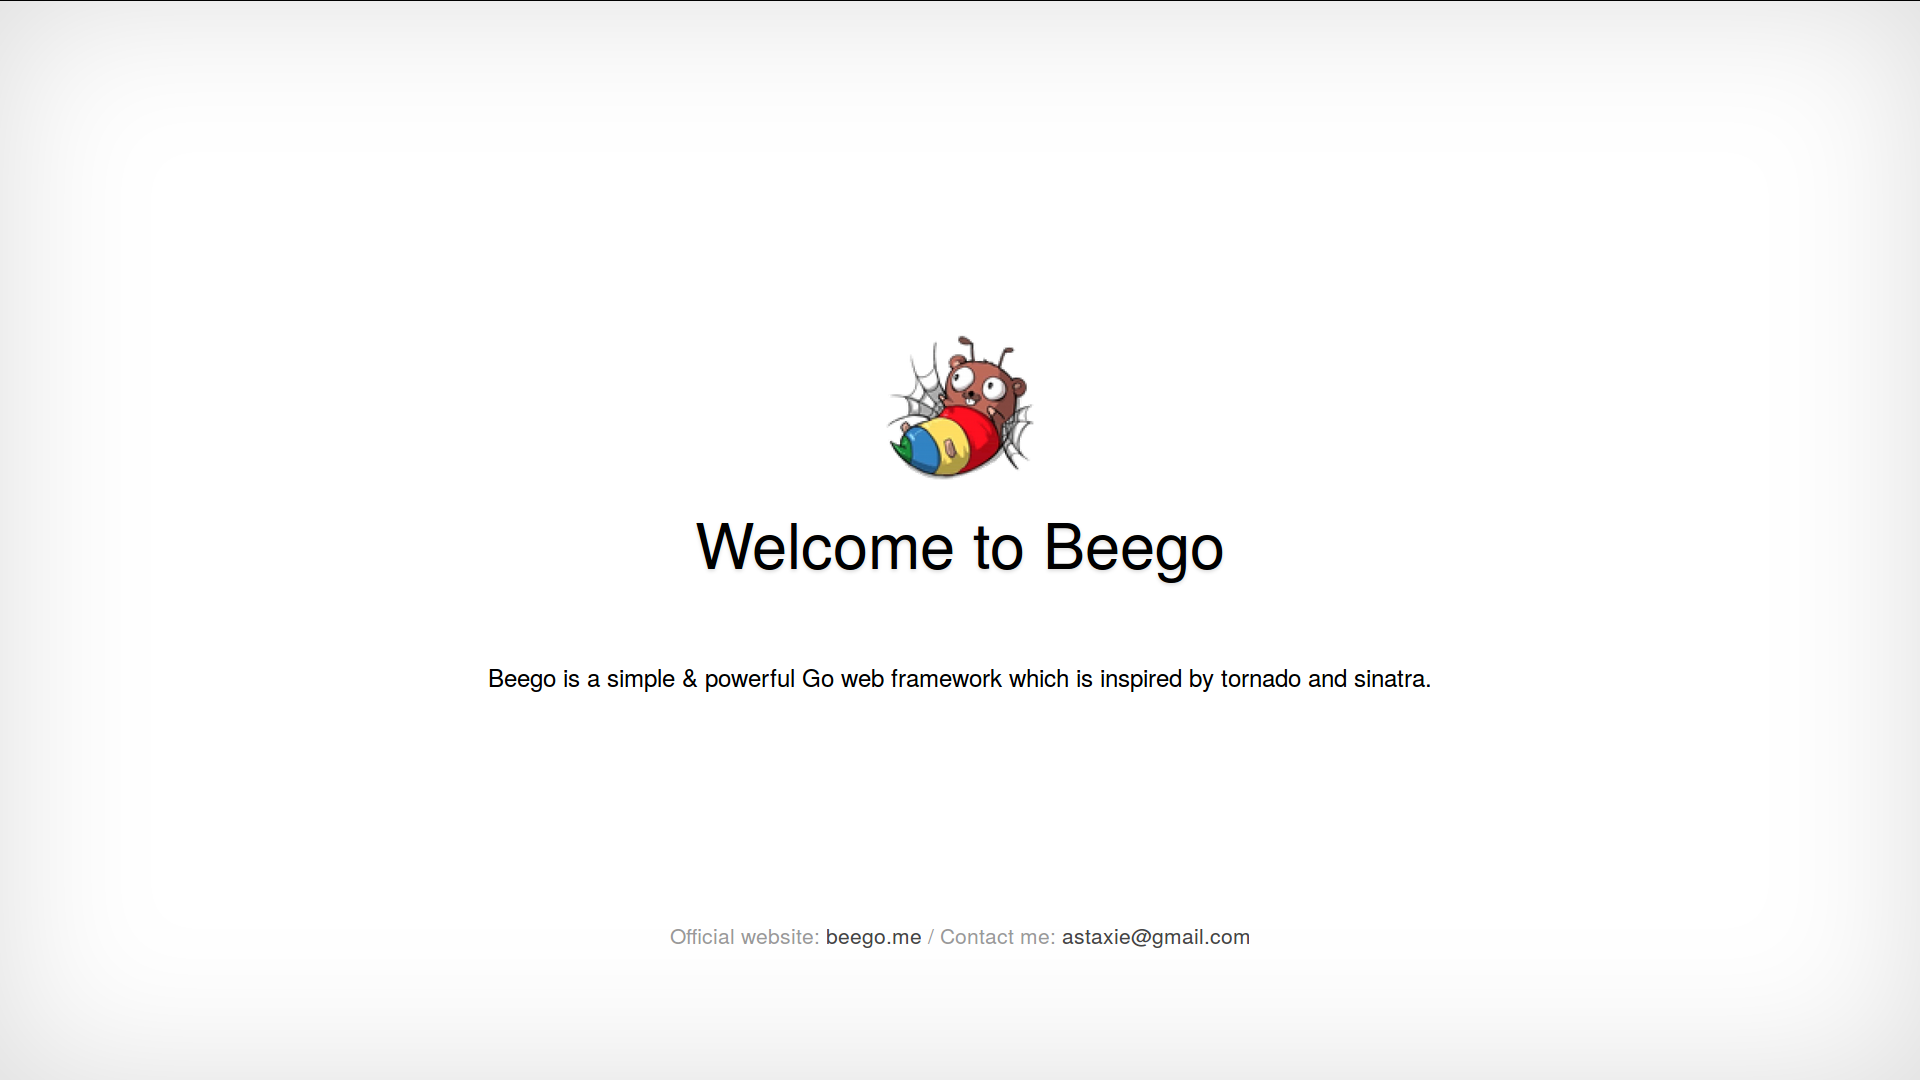
\includegraphics[scale=0.25]{beego.png}

\end{document}
